\documentclass[12pt]{article}
\usepackage[a4paper, total={6in, 9in}]{geometry}
\usepackage{graphicx}
\graphicspath{ {./images/output/} }
\usepackage{caption}
\usepackage[english]{babel}
\usepackage{titling}
\usepackage{float}
\usepackage{amsmath}
\usepackage{minted}
\usepackage{multicol}
% \usepackage{makecell}
\usepackage{tabularx}
\usepackage{multirow}
\usepackage{adjustbox}
% \usepackage{array}
% \usepackage{setspace}
% \usepackage{placeins}
\setlength{\parindent}{0pt}

% \usepackage{lipsum}

\title{Study of Time Division Multiplexing (TDM) \& De-multiplexing}
\author{}
\date{}

\pagenumbering{gobble}
\begin{document}
\vspace*{\fill}
\begin{center}

    \emph{Heaven's Light is Our Guide} \\
    \textbf{Rajshahi University of Engineering and Technology} \\

    \begin{figure}[H]
        \centering
        
\includegraphics[scale=.34]{images/RUET_logo.png}
        \label{fig:ruet_logo}
    \end{figure}
    \vspace{5mm}

    \textbf{Course Code}\\
    ECE 3208\\
    \vspace{3mm}
    \textbf{Course Title}\\
    Communication Engineering Sessional

    \vspace{5mm}
    \textbf{Experiment Date:} {January 21, 2025},\\
    \textbf{Submission Date:} {February 11, 2025}\\

    \vspace{5mm}
    \textbf{Lab Report 3: \\
        Determination of Modulation Index of FM Wave}

    \vspace{15mm}

    \begin{tabular}{c|c}
        \textbf{Submitted to} & \textbf{Submitted by} \\
        Dr. Md. Kamal Hosain  & Md. Tajim An Noor     \\
        Professor             & Roll: 2010025         \\
        Dept of ETE, RUET     &                       \\
    \end{tabular}

\end{center}
\vspace*{\fill}


\pagebreak

\tableofcontents

\pagebreak
\pagenumbering{arabic}
\maketitle

\section*{Theory}
\addcontentsline{toc}{section}{Theory}
Time Division Multiplexing (TDM) allows multiple message signals to share a common communication channel by dividing time into slots, each allocated to a different signal \cite{proakis_digital_communications}. This technique maximizes bandwidth utilization by ensuring each signal gets a dedicated time slot for transmission. Initially, each message signal is filtered to limit its bandwidth, preventing interference with other signals. The signals are then sampled at a rate slightly higher than the Nyquist rate to avoid aliasing and ensure accurate reconstruction at the receiver \cite{oppenheim_signals_systems}.
\\\\
The sampled signals are interleaved in time by a commutator, assigning each sample to a specific time slot. This interleaving allows simultaneous transmission of multiple signals over a single channel without interference. At the receiver, a decommutator separates the interleaved samples, assigning them back to their respective message signals \cite{haykin_communication_systems}.
\\\\
Reconstructing the original message signals from the separated samples is achieved using low-pass filters that smooth out the samples and recreate the continuous-time signals. Synchronization between the commutator and decommutator is essential for proper TDM functioning. Any misalignment can lead to errors in the reconstructed signals, making synchronization mechanisms critical \cite{sklar_digital_communications}. Overall, TDM is a powerful technique enabling efficient and reliable communication in various applications, including telecommunications and data networks.


\section*{Required Apparatus}
\addcontentsline{toc}{section}{Required Apparatus}
\begin{itemize}
    \item TDM Pulse Amplitude Modulation/Demodulation Kit
    \item Oscilloscope
    \item Connecting Wires
    \item Power Supply
\end{itemize}

\section*{Diagrams}
\addcontentsline{toc}{section}{Diagrams}
\subsection*{Block Diagram of TDM System}
\begin{figure}[H]
    \centering
    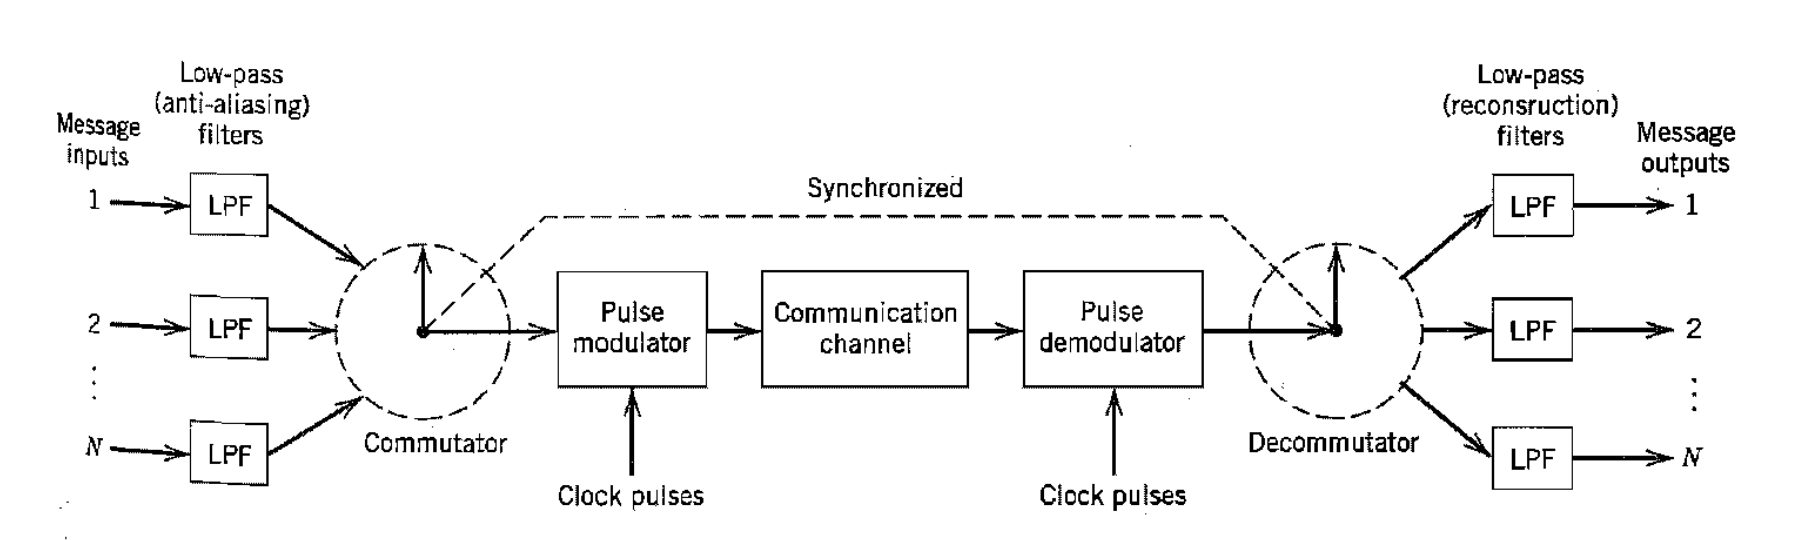
\includegraphics[width=.95\textwidth]{ckt.png}
    \caption{Block Diagram of TDM System \cite{haykin_communication_systems}}
    \label{fig:ckt}
\end{figure}

\subsection*{Circuit Connection of the Kit}
\begin{figure}[H]
    \centering
    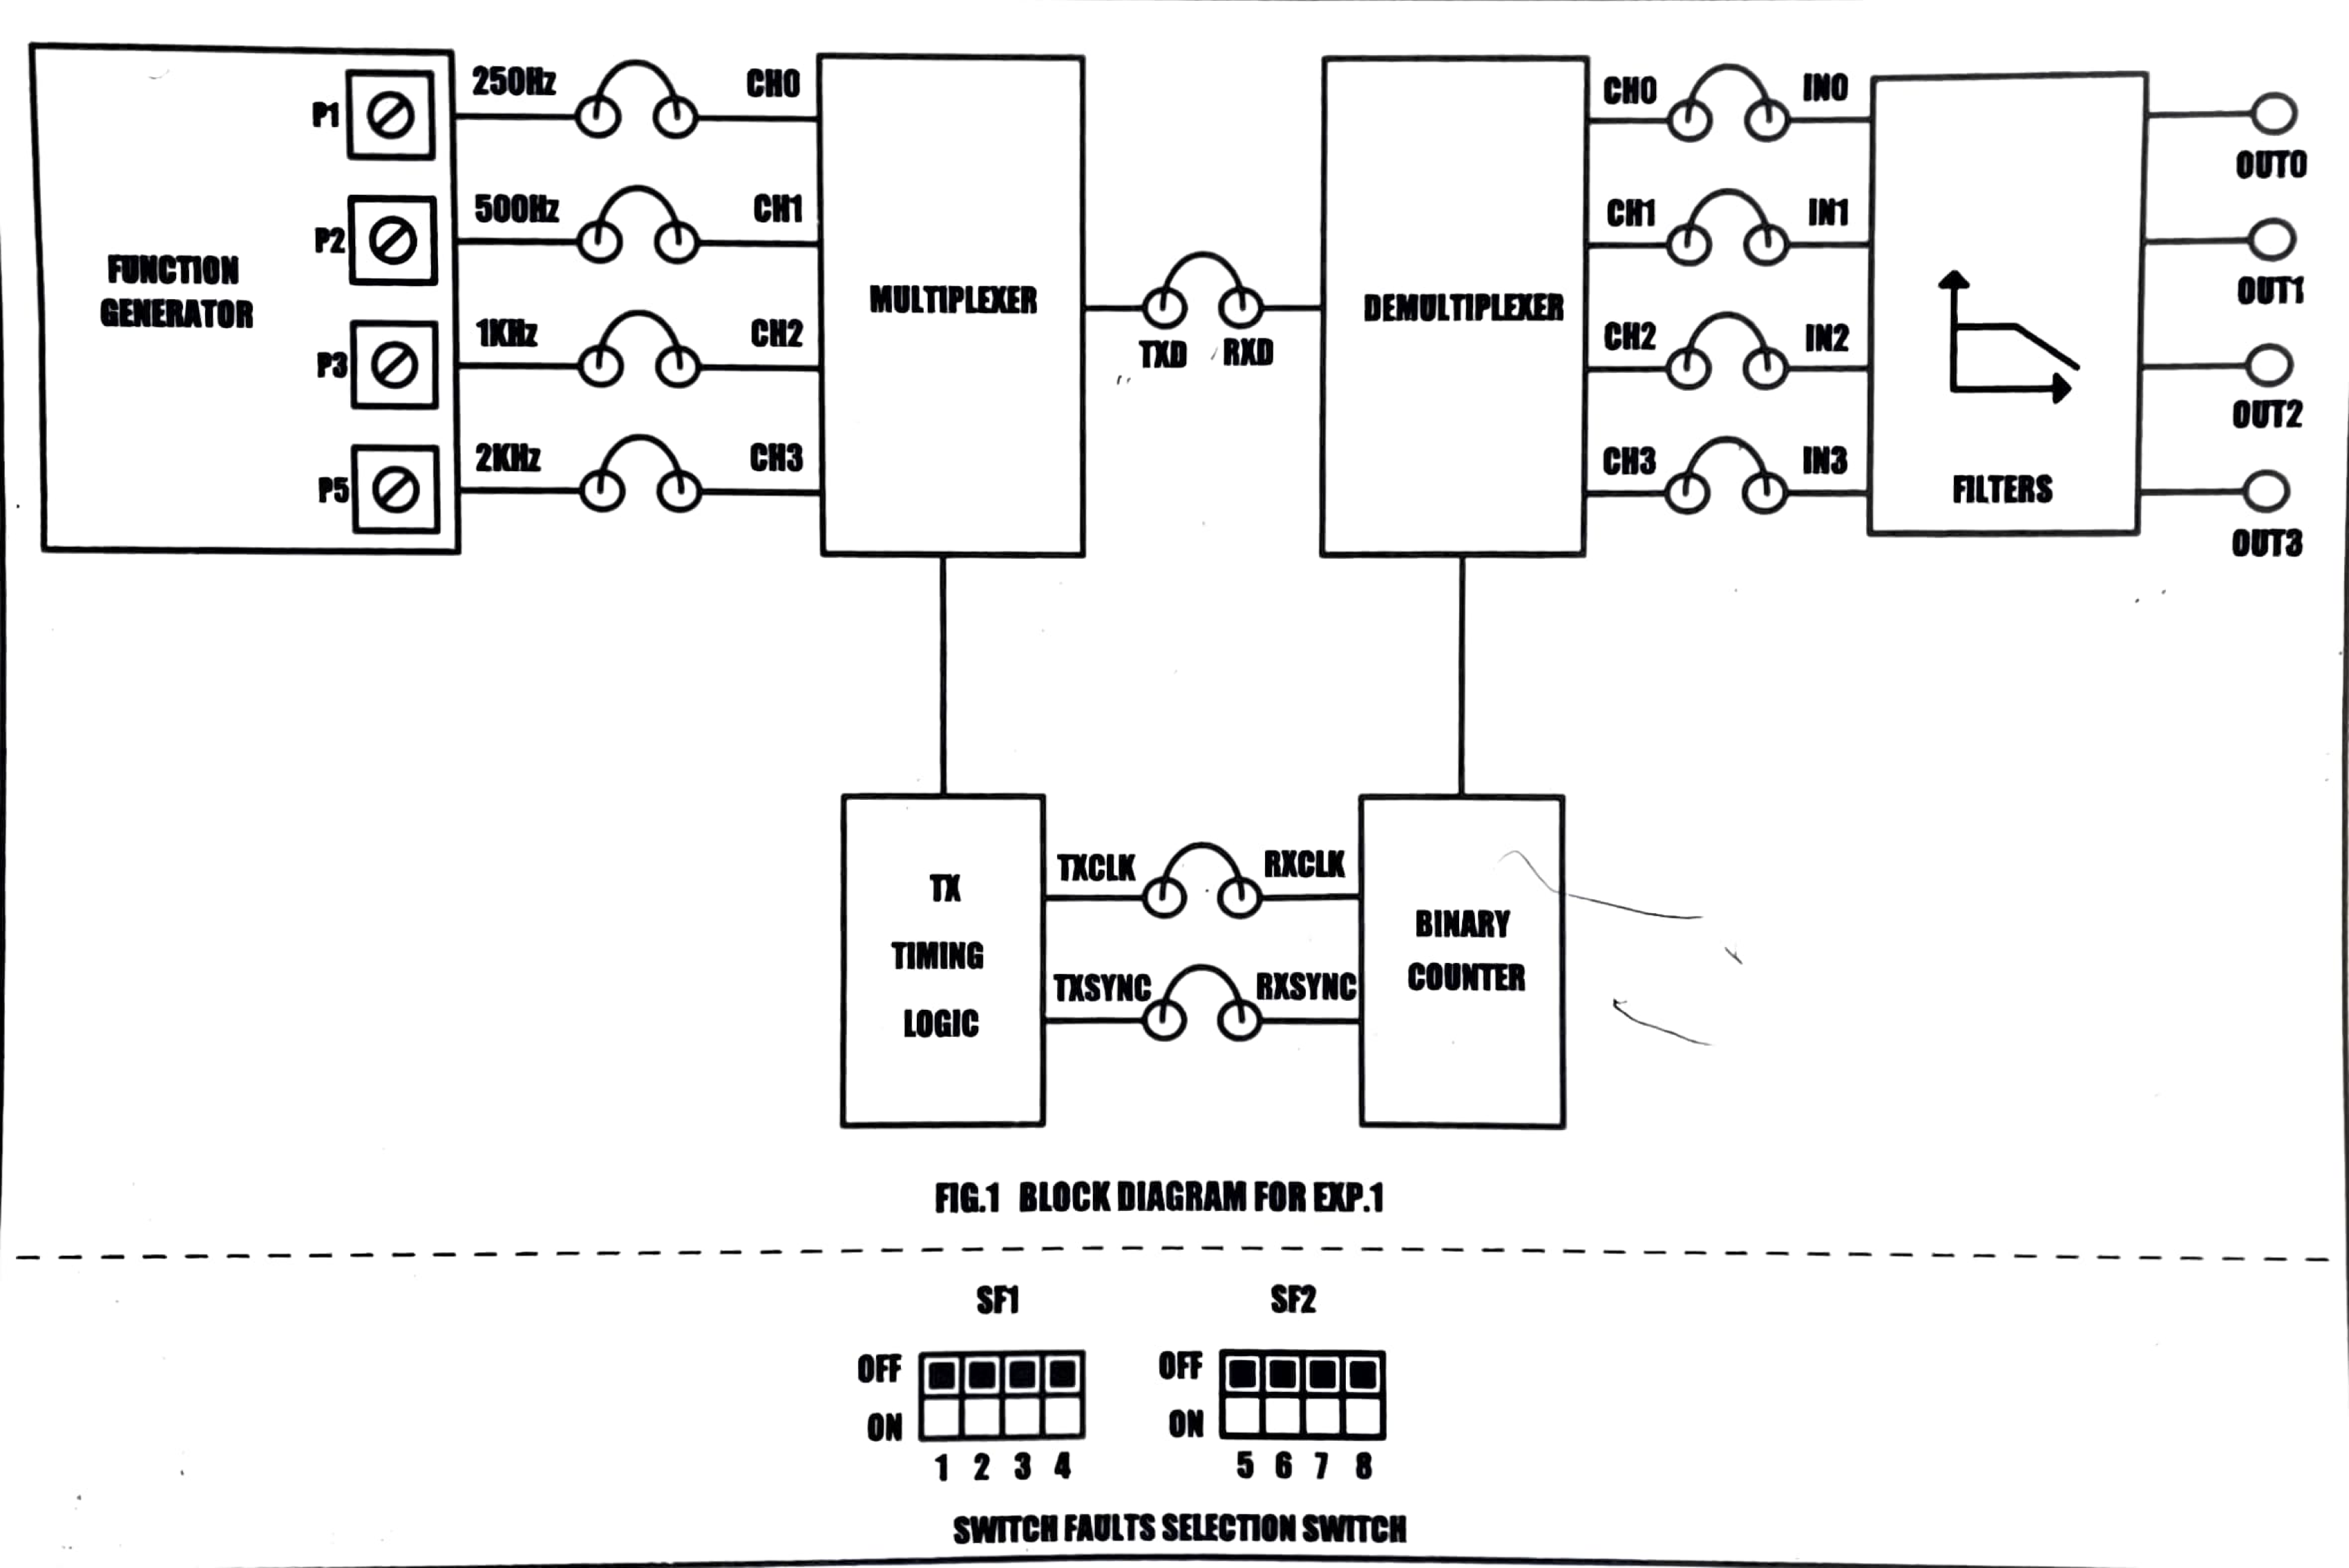
\includegraphics[width=.8\textwidth]{kit.png}
    \caption{Circuit Connection of the TDM Kit}
    \label{fig:circuit_connection}
\end{figure}

\section*{Procedure}
\addcontentsline{toc}{section}{Procedure}
\begin{enumerate}
    \item The TDM pulse amplitude modulation/demodulation kit was set up and connected to the power supply.
    \item The oscilloscope was connected to the output ports of the kit to visualize the signals.
    \item The kit was configured to use 5 sources for the TDM process.
    \item 4 different signals were selected from the available sources.
    \item The selected signals were passed through the multiplexer on the kit.
    \item Observe the output message at different ports using the oscilloscope.
    \item Record the observations and ensure the signals are correctly multiplexed and de-multiplexed.
\end{enumerate}


\section*{Experimental Data}
\addcontentsline{toc}{section}{Experimental Data}
\begin{table}[H]
    \centering
    \begin{tabular}{|c|c|}
        \hline
        \textbf{Signal Number} & \textbf{Frequency (Hz)} \\
        \hline
        1                      & 250                     \\
        \hline
        2                      & 500                     \\
        \hline
        3                      & 1000                    \\
        \hline
        4                      & 2000                    \\
        \hline
    \end{tabular}
    \caption{Message Signal Frequencies}
    \label{tab:signal_frequencies}
\end{table}

\section*{Observation}
\addcontentsline{toc}{section}{Observation}
\begin{enumerate}
    \item The message signal was observed using the oscilloscope.
    \item The multiplexed signal was visualized on the oscilloscope.
    \item The de-multiplexed signal was also observed using the oscilloscope.
    \item Finally, the output message signal was checked using the oscilloscope.
    \item Some faults in the kit were noted, so the outputs were not accurate.
\end{enumerate}

\section*{Matlab Simulation}
\addcontentsline{toc}{section}{Matlab Simulation}

\subsection*{Code:}
\addcontentsline{toc}{subsection}{Code}

\inputminted[linenos,breaklines,breakanywhere]{matlab}{./assets/tdm.m}

\section*{Output}
\addcontentsline{toc}{section}{Output}

\subsection*{Experimental Output}
\addcontentsline{toc}{subsection}{Experimental Output}
\begin{figure}[H]
    \centering
    \begin{minipage}{0.45\linewidth}
        \centering
        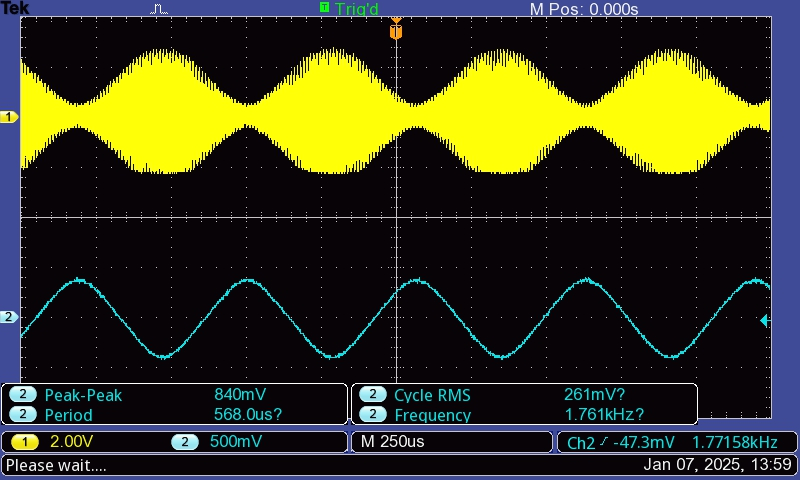
\includegraphics[width=\linewidth]{p1-undMod-msg.JPG}
        \caption{AM; Yellow: Under-modulated, Blue: Message}
        \label{fig:pic1}
    \end{minipage}
    \hfill
    \begin{minipage}{0.45\linewidth}
        \centering
        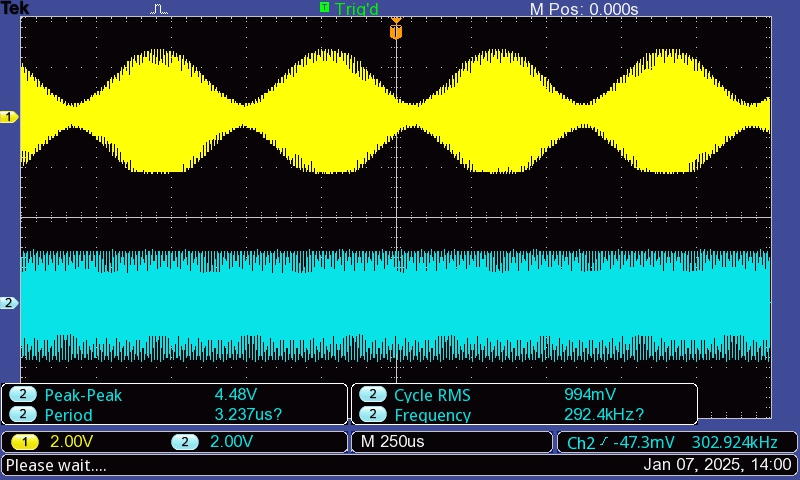
\includegraphics[width=\linewidth]{p2-undMod-car.JPG}
        \caption{AM; Yellow: Under-modulated, Blue: Carrier}
        \label{fig:pic2}
    \end{minipage}
    \vspace{1em}
    \begin{minipage}{0.45\linewidth}
        \centering
        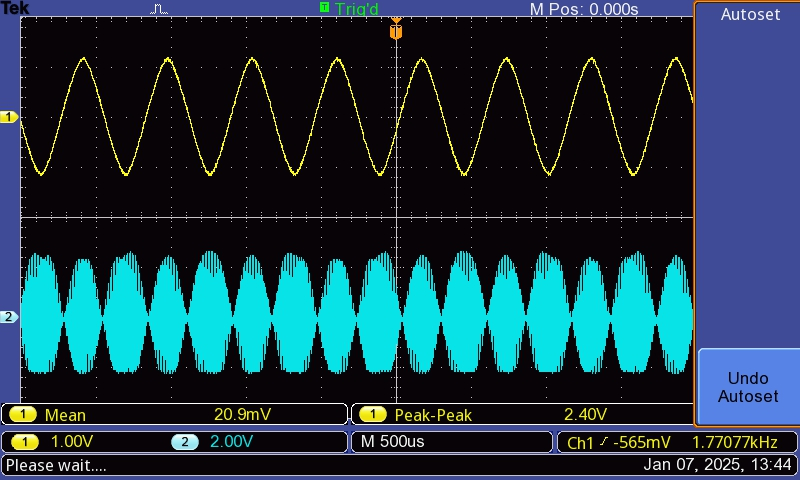
\includegraphics[width=\linewidth]{p3-msg-100mod.JPG}
        \caption{AM; Yellow: Message, Blue: 100\% Modulated}
        \label{fig:pic3}
    \end{minipage}
    \hfill
    \begin{minipage}{0.45\linewidth}
        \centering
        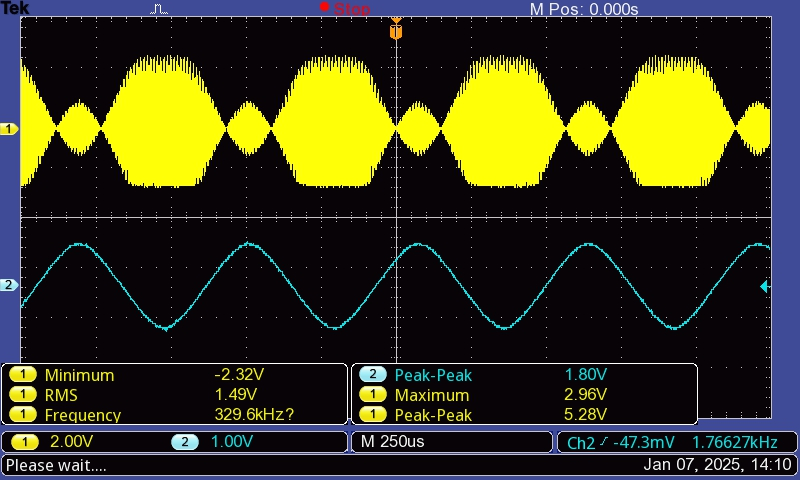
\includegraphics[width=\linewidth]{p4-ovMod-msg.JPG}
        \caption{AM; Yellow: Over-modulated, Blue: Message}
        \label{fig:pic4}
    \end{minipage}
    \vspace{1em}
    \begin{minipage}{0.45\linewidth}
        \centering
        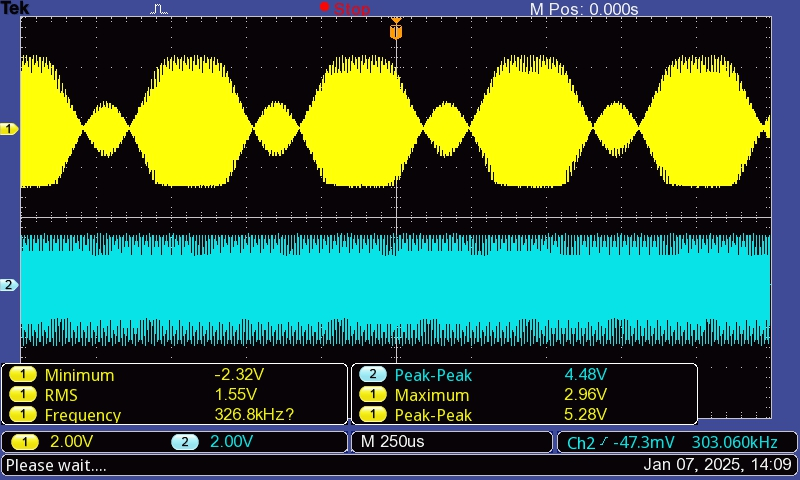
\includegraphics[width=\linewidth]{p5-ovMod-car.JPG}
        \caption{AM; Yellow: Over-modulated, Blue: Carrier}
        \label{fig:pic5}
    \end{minipage}
    \hfill
    \begin{minipage}{0.45\linewidth}
        \centering
        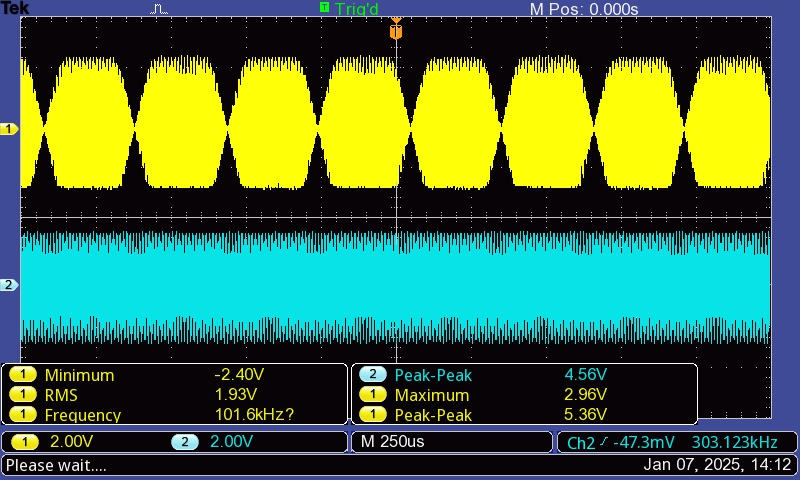
\includegraphics[width=\linewidth]{p6-dsb-mod-car.JPG}
        \caption{DSB\-SC; Yellow: Modulated, Blue: Carrier}
        \label{fig:pic6}
    \end{minipage}
\end{figure}

\pagebreak

\begin{figure}[H]
    \centering
    \begin{minipage}{0.45\linewidth}
        \centering
        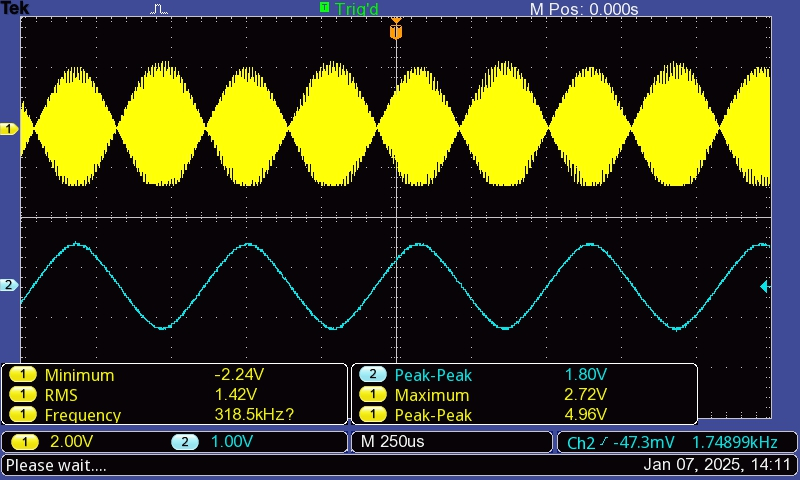
\includegraphics[width=\linewidth]{p7-dsb-mod-msg.JPG}
        \caption{DSB\-SC; Yellow: Modulated, Blue: Message 1}
        \label{fig:pic7}
    \end{minipage}
    \hfill
    \begin{minipage}{0.45\linewidth}
        \centering
        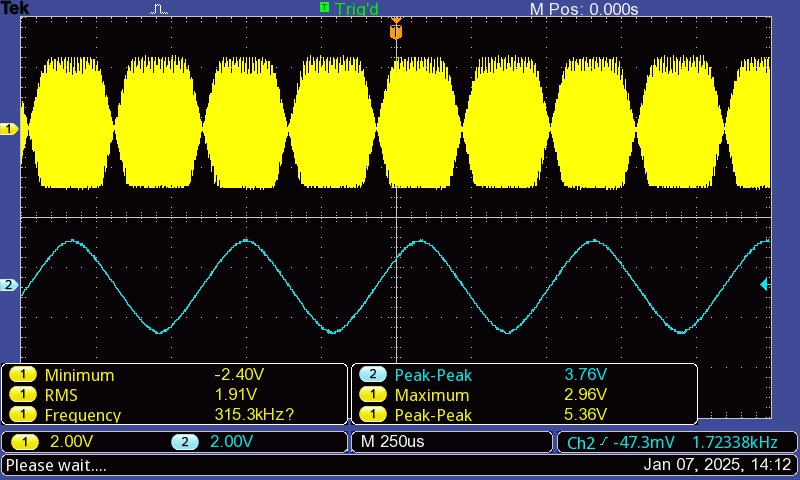
\includegraphics[width=\linewidth]{p8-dsb-mod-msg2.JPG}
        \caption{DSB\-SC; Yellow: Modulated, Blue: Message 2}
        \label{fig:pic8}
    \end{minipage}
    \vspace{1em}
    \begin{minipage}{\linewidth}
        \centering
        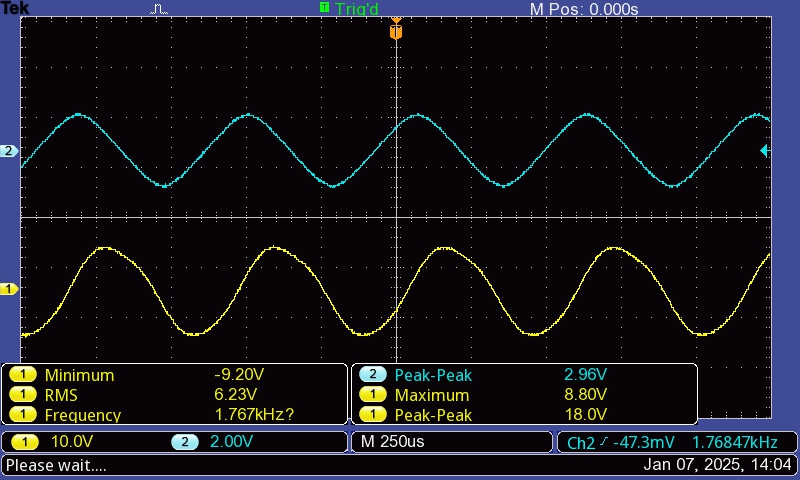
\includegraphics[width=0.4\linewidth]{p9-dsb-msg-Demod.JPG}
        \caption{DSB\-SC; Yellow: Message, Blue: Demodulated Message}
        \label{fig:pic9}
    \end{minipage}
\end{figure}

\subsection*{Matlab Simulation Output}
\addcontentsline{toc}{subsection}{Matlab Output}
\begin{figure}[H]
    \centering
    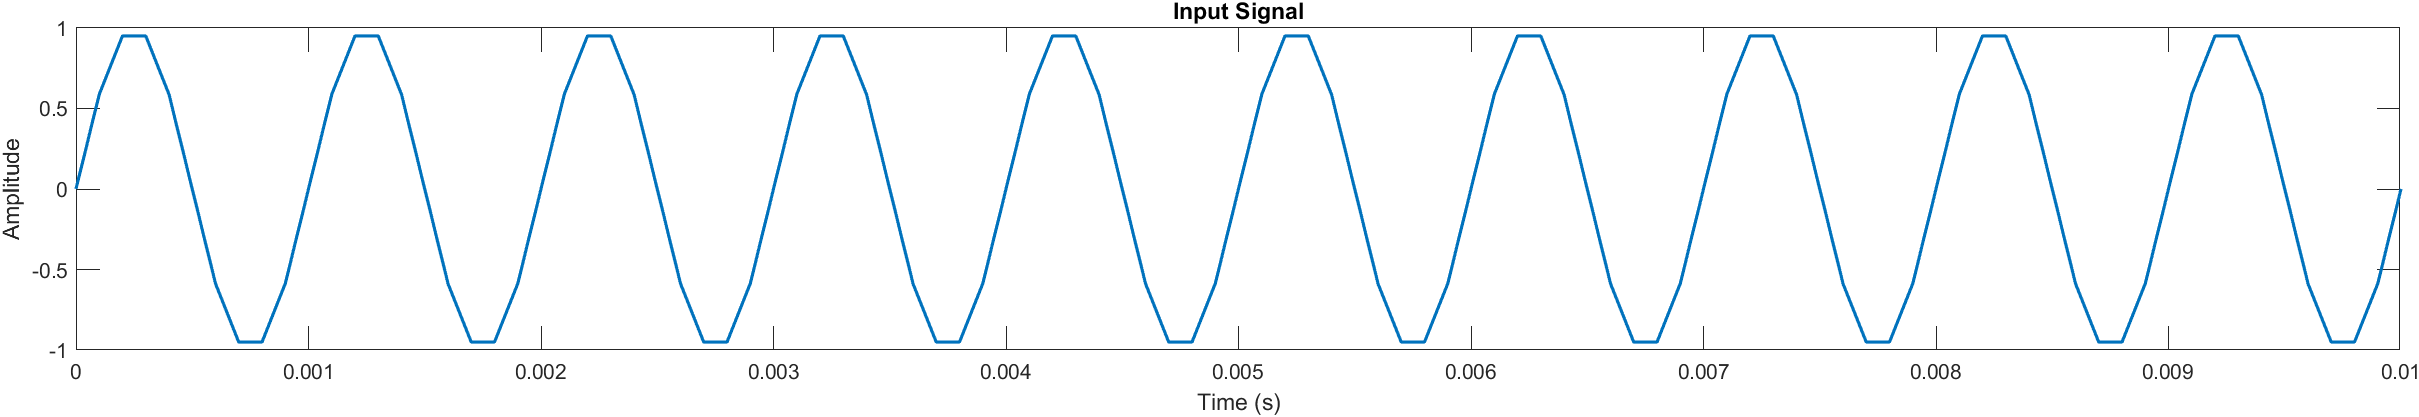
\includegraphics[width=\textwidth]{msg.png}
    \caption{Message Signal}
    \label{fig:img2}
\end{figure}

\begin{figure}[H]
    \centering
    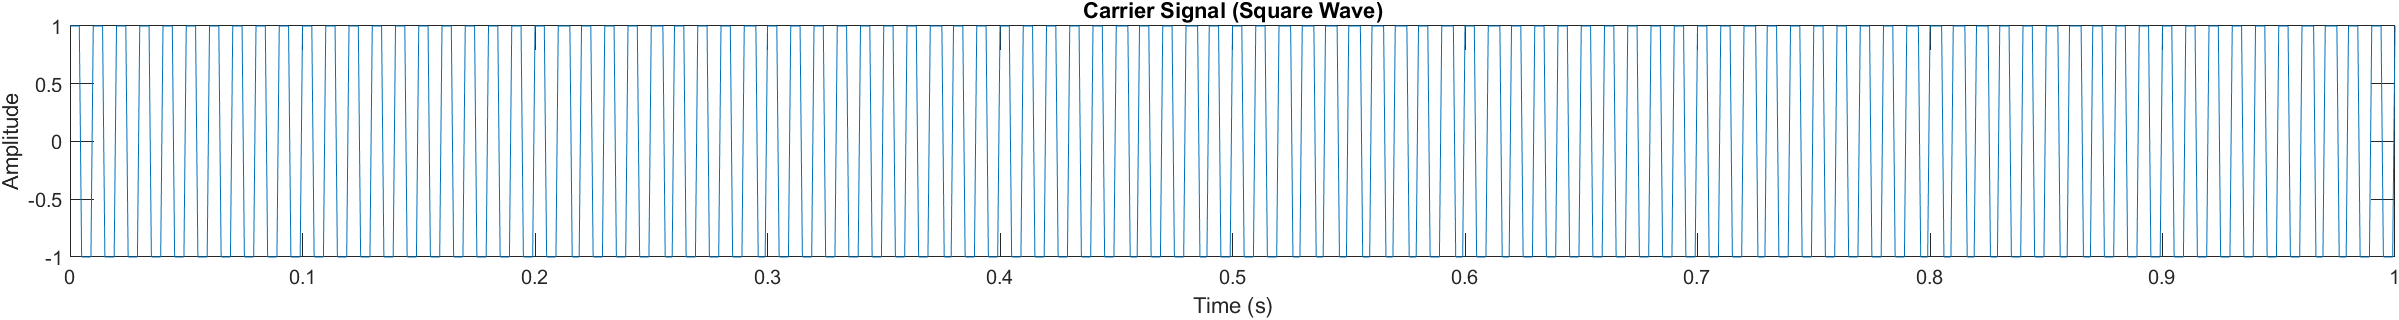
\includegraphics[width=\textwidth]{car.png}
    \caption{Carrier Signal, Square Wave}
    \label{fig:img11}
\end{figure}

\begin{figure}[H]
    \centering
    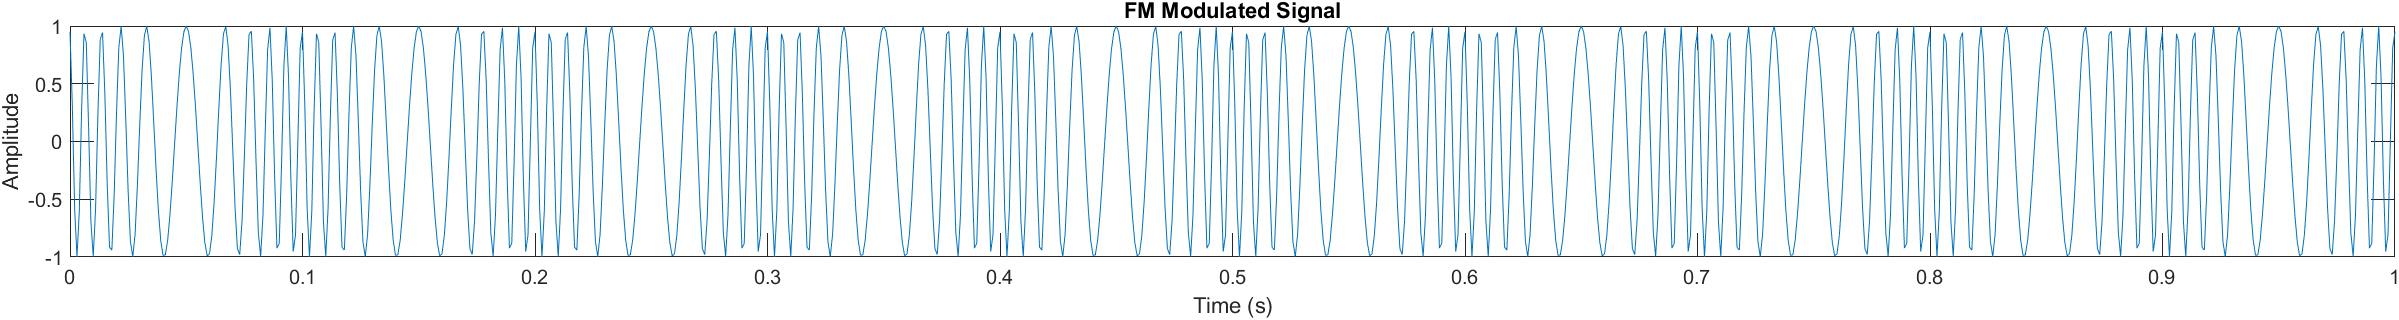
\includegraphics[width=\textwidth]{mod.png}
    \caption{FM Modulated Signal}
    \label{fig:img3}
\end{figure}

\begin{figure}[H]
    \centering
    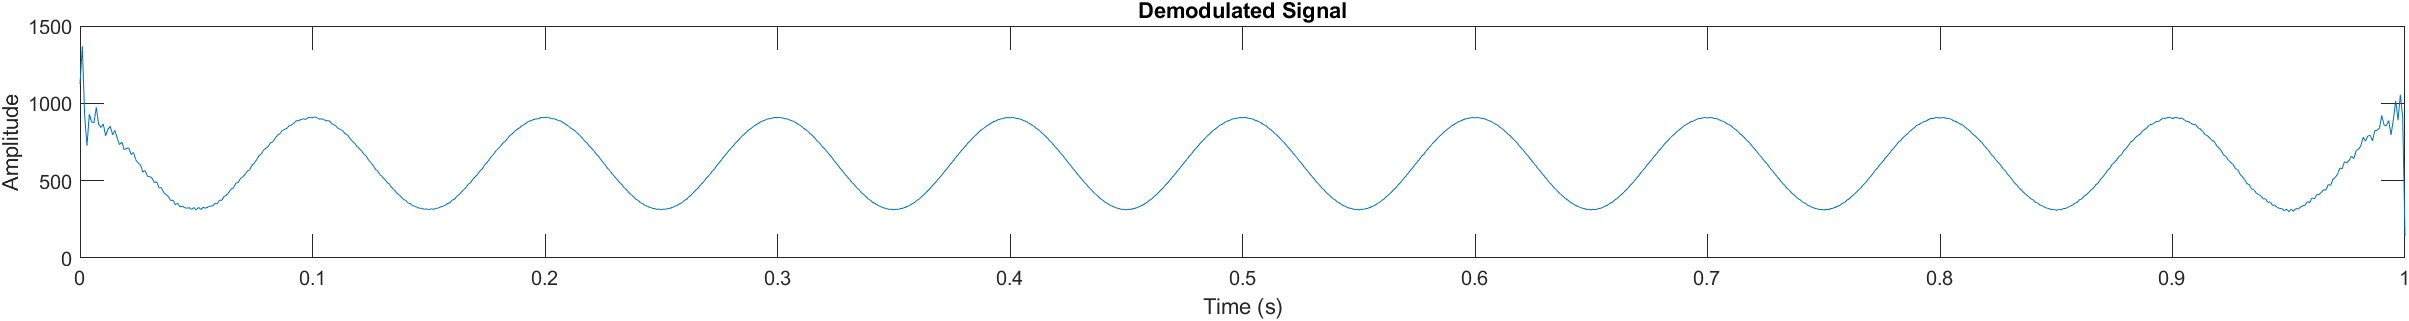
\includegraphics[width=\textwidth]{demod.png}
    \caption{Demodulated Signal}
    \label{fig:img4}
\end{figure}


\section*{Discussion and Conclusion}
\addcontentsline{toc}{section}{Discussion and Conclusion}
In this experiment, we explored the principles and practical implementation of Time Division Multiplexing (TDM) and De-multiplexing. Using a TDM Pulse Amplitude Modulation/Demodulation Kit and an oscilloscope, we observed the multiplexing and de-multiplexing processes. The oscilloscope visualized the signals at various stages, and despite some inaccuracies due to faults in the kit, the experiment effectively demonstrated the fundamental concepts of TDM. The Matlab simulation provided additional insights, with the simulation output aligning with theoretical expectations.
\\\\
In conclusion, this experiment offered valuable insights into TDM and its practical applications. The combination of theoretical study, hands-on experimentation, and Matlab simulation provided a comprehensive understanding of the topic. Future experiments could focus on addressing the kit's faults for more accurate results and exploring advanced TDM techniques for complex communication systems.

\bibliographystyle{IEEEtran}
\renewcommand{\bibname}{References}
\addcontentsline{toc}{section}{References}
\bibliography{ref}

\end{document}
